\documentclass{article}
\usepackage[utf8]{inputenc}
\usepackage[margin=1in]{geometry}
\usepackage{amsmath}
\usepackage{amsthm}
\usepackage{mathtools}
\usepackage{verbatim}
\DeclareMathOperator{\sech}{sech}
\usepackage{braket}
\usepackage{bbold}
\usepackage{graphicx}
\usepackage{xcolor}
\usepackage{import}
\usepackage{xifthen}
\usepackage{pdfpages}
\usepackage{transparent}

\newcommand{\incfig}[1]{%
    \def\svgwidth{10cm}
    \import{./Figures/}{#1.pdf_tex}
}

\newcommand{\incfigsize}[2]{%
    \def\svgwidth{#2cm}
    \import{./Figures/}{#1.pdf_tex}
}

\graphicspath{{./Mathematica/}}
\title{Tunnelling Times in Quantum Mechanics}
\author{James Puleston}

\begin{document}

\maketitle

\section{Time in Quantum Mechanics}

\subsection{Time in Classical Mechanics}
In the Hamiltonian formulation of classical mechanics, a system with $n$ degrees of freedom possesses $2n$ independent first-order differential equations in terms of $2n$ independent variables. These variables are the coordinates of the \textit{phase space} of the system, and the $2n$ equations of motion describe the evolution of system in the phase space. $n$ of the independent variables are conventionally chosen to be the generalised coordinates $q_i$ and the other $n$ set to be the conjugate momenta $p_i$, which obey the Poisson bracket relations (Goldstein 2002):

\begin{equation}
	\{q_i, p_j\}=\delta_{ij} \quad \{q_i, q_j\}=\{p_i,p_j\}=0, \quad i,j=\{1,\dots,n\}.
	\label{conjugatevars}
\end{equation}

\noindent The time evolution of the canonical variables is governed by the Hamiltonian $H = H(q_i, p_i)$:

\begin{equation}
	\frac{dq_i}{dt} = \{q_i, H\} \quad \frac{dp_i}{dt} = \{p_i, H\}.
	\label{timeevolution}
\end{equation}

\noindent For an infinitesimal variation in time, $\delta t = \delta \tau$, the associated variation in the dynamical variables is:

\begin{equation}
	\delta q_i = \{q_i, H\}\delta\tau \quad \delta p_i = \{p_i, H\}\delta\tau.
	\label{timetranslation}
\end{equation}

\noindent $q_i$ and $p_i$ are generalised variables; they are not necessarily positions and momenta, but in the case of a dynamical system comprised of a collection of point particles, the canonical variables are usually the particles' positions $(\boldsymbol{q_i})$ and momenta $(\boldsymbol{p_i})$. 

In classical mechanics, physical systems are embedded in a 4-dimensional continuous space-time background, the points of which are assigned coordinates $(t,x,y,z) = (t, \boldsymbol{x})$.
It is essential that the \textit{definitions} of these two spaces and their associated coordinates are not conflated (Hilgevoord 2002). In particular we must distinguish the position variable $\boldsymbol{q}$ from the space-time coordinate $\boldsymbol{x}$. The former defines a point in the phase space of the system (when accompanied by its associated momentum $\boldsymbol{p}$) and is a property of a point particle, whereas the latter is the coordinate of a fixed point in the space-time background in which the dynamical system is embedded. Note that we can still introduce both sets of quantities in to equations and relate them, as equations (\ref{timeevolution}) and (\ref{timetranslation}) show.

Immediately this raises the question of whether there are physical systems that possess a dynamical variable that \textit{resembles} the time coordinate of space-time. Such systems are called \textit{clocks}:, more precisely defined as physical systems with a dynamical `clock' or `time' variable that behaves similarly to the space-time time coordinate $t$ under time translations. For example, under time translation in which the space-time coordinates transform as (cf. Hilgevoord 2002, (9), (10), (11)):

\begin{equation}
\boldsymbol{x} \rightarrow \boldsymbol{x} \quad t \rightarrow t+\tau
\label{timetranslation2}
\end{equation}

\noindent a \textit{linear} clock variable $\theta$ and its conjugate momentum $\eta$ transform as:

\begin{equation}
	\eta \rightarrow \eta \quad \theta \rightarrow \theta + \tau.
	\label{timetranslation3}
\end{equation}

\noindent Comparing with (\ref{timetranslation}) we see in the infinitesimal case of (\ref{timetranslation3}):

\begin{equation}
	\delta\eta=\{\eta, H\}\delta\tau \quad \delta\theta = \{\theta, H\}\delta\tau
	\label{timetranslation4}
\end{equation}

\noindent which implies

\begin{equation}
	\{\eta, H\}=0 \quad \{\theta, H\}=1.
	\label{timetranslation5}
\end{equation}

\noindent The equation of motion given by (\ref{timeevolution}), $d\theta/dt=1$ has solution $\theta=t+t_0$.

\subsection{Time in Quantum Mechanics}
In quantum mechanics the state of a particle is encoded in a vector $\ket{\psi}$ in Hilbert space $\mathcal{H}$. Introducing a 1-dimensional continuum position basis in $\mathcal{H}, \{\ket{q}\}, q \in \mathbb{R}$, the state vector $\ket{\psi}$ can be expanded as the integral (Sakurai 2017):

\begin{equation}
	\ket{\psi} = \int_{\mathbb{R}}dq\psi(q)\ket{q}
\end{equation}

\noindent where $\psi(q)$ is the wave function of the particle. More generally, to describe a system in 3 dimensions requires a wave function $\psi(q_x,q_y,q_z)$. It is important to note that the domain of the wave function is the \textit{configuration space} of the system, $\mathbb{R}^3$, whose coordinates are the generalised coordinates $q_i$ of the system. It is common in elementary quantum mechanics literature for elements of the domain of the wave function to be expressed as $(x,y,z), \text{ i.e. } \psi = \psi(x,y,z)$. This is clearly in notational conflict with the use of $(x,y,z)$ as coordinates of points of the background space-time in which the quantum system resides. In agreement with the literature surveyed in this essay I retain this notation throughout; but the distinction between space-time coordinates and dynamical variables should be maintained.

Measurable quantities or `observables' are represented by operators on $\mathcal{H}$:

\begin{equation}
	\mathcal{O}: \mathcal{H} \rightarrow \mathcal{H}.
\end{equation}

\noindent Such operators arise through a procedure called `canonical quantisation', which prescribes that \textit{dynamical variables} of the Hamiltonian formalism are promoted to operators on $\mathcal{H}$ and their Poisson bracket relations replaced by commutation relations according to:

\begin{equation}
\{\cdot,\cdot\} \rightarrow \frac{1}{i\hbar}[\cdot,\cdot].
\end{equation}

\noindent One notable omission in this process is the promotion of the time coordinate $t$ to an operator. Given the emphasis placed on distinguishing between space-time coordinates and dynamical variables, the reason is clear: time $t$ is a \textit{space-time coordinate}, and canonical quantisation prescribes that \textit{dynamical variables} are promoted to operators. However this raises the question of whether a time operator exists in quantum mechanics. The resolution of this problem has been historically hindered by a `proof' offered by Wolfgang Pauli showing that the introduction of a time operator in quantum mechanics is forbidden. It proceeds roughly along the following lines:

\textcolor{red}{Add Pauli proof c.f. Butterfield On Time in Quantum Physics}

Observing that this issue arose from attempts to erroneously quantise the \textit{space-time} coordinate $t$, the problem becomes void such that progress can be made by considering the quantisation of timelike \textit{dynamical variables} of physical systems, namely clocks in analogy with the case in classical mechanics mentioned above. 

Despite this clarification, approaches to the question \textit{how long does a quantum particle take to tunnel through a classically forbidden potential barrier?} have not yielded a satisfactory answer that is universally agreed upon by the physics community. The question can be more formally posed as \textit{when a particle with energy less than the barrier potential traverses the barrier region and is ultimately transmitted, how much time did it, on average, spend in the barrier region?} 

Many solutions to this question have been offered within the orthodox interpretation of quantum mechanics. In section \ref{subsection:quantumbarrier} I describe the physical system (quantum tunnelling experiment) of interest, and in sections \ref{subsection:phasetime}-\ref{subsection:larmorprecession} I survey definitions within the orthodox viewpoint. However, the de Broglie-Bohm interpretation of quantum mechanics offers a clear and unambiguous answer to the question at hand, so in section \ref{subsection:dBBtheory} I introduce the requisite theory, in section \ref{subsection:dBBtime} I present the natural definition of tunnelling time within the de Broglie-Bohm interpretation, and in section \ref{subsection:dBBexample} I conclude with a numerical analysis of a quantum tunnelling experiment.

\section{Tunnelling Times in the Orthodox Interpretation}
\label{section:Orthodox}

In this section I survey a number of contenders for calculating the tunnelling time through a barrier. The definitions in sections \ref{subsection:phasetime}-\ref{subsection:dcqc} are `intrinsic' quantities, in that they make no reference to a measuring apparatus (other than the implied particle detector to determine whether or not an incident particle is eventually transmitted) (Leavens 1996). Section \ref{subsection:larmorprecession} offers an `experimental' definition, making reference to a specific physical system.

Throughout this essay I use the physical system described in (B{\"u}ttiker 1983). The systems used in other literature surveyed in this essay differ by choice of coordinates and/or barrier location and I have accordingly recalculated various quantities throughout the essay for the physical system used by B{\"u}ttiker and myself.

\subsection{Tunnelling Through a Quantum Barrier}
\label{subsection:quantumbarrier}

\noindent Consider the case of scattering in one dimension with particles of mass $m$, velocity $v(k) = \hbar k/m$ and kinetic energy $E = \hbar^2k^2/2m$. The particles move in the positive $y$ direction and interact with a rectangular barrier:

\begin{equation}
	V = 
	\begin{cases}
	V_0 & -\frac{d}{2}<y<\frac{d}{2}\\
		0 & \text{otherwise}
	\end{cases}
\end{equation}

\begin{figure}[ht]
    \centering
    \incfig{potentialbarrier}
    \caption{The quantum potential barrier}
    \label{fig:potentialbarrier}
\end{figure}

\noindent Note that $E<V_0$ so that this system describes a quantum tunnelling experiment.

\noindent The wave function is of the form:
\begin{equation}
	\psi(y,k) = 
	\begin{cases}
		e^{iky} + Ae^{-iky} & y \leq -\frac{d}{2} \\
		Be^{\kappa y} + Ce^{-\kappa y} & -\frac{d}{2} \leq y \leq \frac{d}{2} \\
		De^{iky} & y \geq \frac{d}{2}
	\end{cases}
	\label{wavefunction}
\end{equation}
\noindent where $k = \sqrt{2mE}/\hbar$, $\kappa := \sqrt{2m(V_0-E)}/\hbar = \sqrt{k_0^2-k^2} \text{ where } k_0 = \sqrt{2mV_0}/\hbar$ and $A,B,C,D$ are functions of the variables of the system.

The coefficient of the incident wave is set to one, corresponding to one particle per unit length in the incident beam. Note there is no $e^{-iky}$ term on the right of the barrier, as no particles are reflected after being transmitted through the barrier.

\noindent Calculation of the wave function coefficients $A,B,C,D$ uses the continuity of the wave function and its first derivative at the barrier boundaries. The results are frequently stated without proof in the literature, but will be used so frequently in this essay that I provide a derivation. The results are:

\begin{align}
	D &= T^{\frac{1}{2}}e^{i\Delta\phi}e^{-ikd} & A &= R^{\frac{1}{2}}e^{-i\pi/2}e^{i\Delta\phi}e^{-ikd} \nonumber \\
	B &= \frac{\kappa+ik}{2\kappa}e^{ikd/2}e^{-\kappa d/2}D & C &= \frac{\kappa-ik}{2\kappa}e^{ikd/2}e^{\kappa d/2}D \label{cont0}
\end{align}
where $T$ is the transmission probability, $R = 1-T$ is the reflection probability and $\Delta\phi$ is the phase change across the barrier (calculated below) (B{\"u}ttiker 1983).

\begin{proof}
	\noindent First I introduce a new coordinate system so that the boundaries of the barrier become $0,d \text{ i.e. } \tilde{y} = y+d/2$. Then, denoting the wave functions to the left of, inside, and to the right of the barrier as $\psi_{1}, \psi_{2}, \psi_{3}$ respectively, yields:

\begin{subequations}
\begin{align}
	\psi_{1} &= e^{-ikd/2}e^{ik\tilde{y}} + \tilde{A}e^{-ik\tilde{y}} & \psi_{1}^{'} &= ike^{ikd/2}e^{ik\tilde{y}} - ik\tilde{A}e^{-ik\tilde{y}} \\
	\psi_{2} &= \tilde{B}e^{\kappa\tilde{y}} + \tilde{C}e^{-\kappa\tilde{y}} & \psi_{2}^{'} &= \kappa\tilde{B}e^{\kappa\tilde{y}} -\kappa \tilde{C}e^{-\kappa \tilde{y}} \\
	\psi_{3} &= \tilde{D}e^{ik\tilde{y}} & \psi_{3}^{'} &= ik\tilde{D}e^{ik\tilde{y}}
\end{align}
\label{wavefunctions2}
\end{subequations}

\noindent where $\tilde{A} = Ae^{ikd/2}, \tilde{B} = Be^{-\kappa d/2}, \tilde{C} = Ce^{\kappa d/2}, \tilde{D} = De^{-ikd/2}$.

\noindent Imposing continuity of the wave function and its first derivative at the barrier boundaries:
\begin{subequations}
\begin{align}
	\psi_{1}(0) = \psi_{2}(0) &\implies e^{\frac{-ikd}{2}}+\tilde{A} = \tilde{B}+\tilde{C} \label{cont1}\\
	\psi_{1}^{'}(0) = \psi_{2}^{'}(0) &\implies ike^{\frac{-ikd}{2}} - ik\tilde{A} = \kappa \tilde{B} - \kappa \tilde{C} \label{cont2}\\
	\psi_{2}(d) = \psi_{3}(d) &\implies e^{\kappa d}\tilde{B} + e^{-\kappa d}\tilde{C} = e^{ikd}\tilde{D} \label{cont3}\\
	\psi_{2}^{'}(d) = \psi_{3}^{'}(d) &\implies \kappa e^{\kappa d}\tilde{B} + -\kappa e^{-\kappa d}\tilde{C} = ike^{ikd}\tilde{D} \label{cont4}\\
	\\
	ik(\ref{cont1})+(\ref{cont2}) &\implies 2ike^{-ikd/2} = (ik+\kappa)\tilde{B}+(ik-\kappa)\tilde{C} \label{cont5}\\
	\kappa(\ref{cont3})+(\ref{cont4}) &\implies 2\kappa e^{\kappa d}\tilde{B} = (\kappa+ik)e^{ikd}\tilde{D} \label{cont7}\\
	\kappa(\ref{cont3})-(\ref{cont4}) &\implies 2\kappa e^{-\kappa d}\tilde{C} = (\kappa-ik)e^{ikd}\tilde{D} \label{cont8}.
	\end{align}
\end{subequations}

\noindent Inserting equations (\ref{cont7}) and (\ref{cont8}) into equation (\ref{cont5}) one arrives at:
\begin{subequations}
\begin{align}
	2ike^{-ikd/2} &= -\frac{(ik-\kappa)^2}{2\kappa}e^{(ik+\kappa)d}\tilde{D}+\frac{(ik+\kappa)^2}{2\kappa}e^{(ik-\kappa)d}\tilde{D} \label{cont9} \\
	\implies 4ik\kappa e^{-ikd}e^{-ikd/2} &= \tilde{D}[(k^2-\kappa^2)(e^{\kappa d}-e^{-\kappa d})+2ik\kappa(e^{\kappa d}+e^{-\kappa d})] \label{cont10}\\
						      &= \tilde{D}[2(k^2-\kappa^2)\sinh{\kappa d}+4ik\kappa \cosh{\kappa d}] \label{cont11}.
\end{align}
\end{subequations}

\noindent Hence one arrives at the first result, the transmission probability $T = |\tilde{D}|^2 \;(=|D|^2)$:
\begin{equation}
	T = \left[1+\frac{(k^2+\kappa^2)^2\sinh^2{\kappa d}}{4k^2\kappa^2}\right]^{-1}.
	\label{transmissionprobability}
\end{equation}

\noindent $\tilde{D}$ can be written in polar form $\tilde{D} = |\tilde{D}|e^{i\theta} = T^{\frac{1}{2}}e^{i\theta}$.

\begin{subequations}
\begin{align}
	\tilde{D}&=\frac{2ik\kappa e^{-ikd}e^{-ikd/2}\left[(k^2-\kappa^2)\sinh{\kappa d}-2ik\kappa\cosh{\kappa d}\right]}{(k^2-\kappa^2)^2\sinh^2{\kappa d}+4k^2\kappa^2\cosh^2{\kappa d}}\\
	\implies \theta &= arg(\tilde{D})=\arctan\left(\frac{\operatorname{Im}(\tilde{D})}{\operatorname{Re}(\tilde{D})}\right) = -\frac{3kd}{2}+\arctan\left(\frac{k^2-\kappa^2}{2k\kappa}\tanh{\kappa d}\right) \label{thetaphase}
\end{align}
\end{subequations}
\noindent where first term comes from the exponential terms and the second term from the hyperbolic terms in (\ref{thetaphase}).

\noindent Using the form of $\psi_3$ in (\ref{wavefunctions2}), the transmitted wave function at $\tilde{y} = d$ is:

\begin{equation}
	\psi_3=\tilde{D}e^{ikd} = T^{1/2}e^{i\theta}e^{ikd}	
\end{equation}

\noindent hence the phase at $\tilde{y} =d$ is $\theta + kd$. Similarly using the form of $\psi_1$, the incident wave function at $\tilde{y} = 0$ is:
\begin{equation}
	\psi_1=e^{-ikd/2}
\end{equation}
\noindent hence the phase at $\tilde{y}=0$ is $-kd/2$. The phase change across the barrier is therefore:

\begin{subequations}
\begin{align}
\Delta\phi = \theta + \frac{3kd}{2} = -\frac{3kd}{2}+\arctan\left(\frac{k^2-\kappa^2}{2k\kappa}\tanh{\kappa d}\right)+\frac{3kd}{2} = \arctan\left(\frac{k^2-\kappa^2}{2k\kappa}\tanh{\kappa d}\right). \label{phasechange}
\end{align}
\end{subequations}

\noindent Hence

\begin{subequations}
\begin{align}
\tilde{D} &= T^{\frac{1}{2}}e^{i\Delta\phi}e^{-3ikd/2}\\
	D&=T^{\frac{1}{2}}e^{i\Delta\phi}e^{-ikd}.
\end{align}
\end{subequations}

\noindent The result for $A$ follows along similar lines and results for $B \text{ and } C$ follow immediately from equations (\ref{cont7}) and (\ref{cont8}).
\end{proof}

\begin{comment}
\begin{proof}	\noindent First I introduce a new coordinate system so that the boundaries of our barrier become $0,d \text{ i.e. } \tilde{y} = y+\frac{d}{2}$. Then, denoting the wave functions to the left of, inside and to the right of the barrier as $\psi_{1}, \psi_{2}, \psi_{3}$ respectively, yields:

\begin{subequations}
\begin{align}
	\psi_{1} &= e^{iky} + Ae^{-iky} & \psi_{1}^{'} &= ike^{iky} - ikAe^{-iky} \\
	\psi_{2} &= Be^{-\kappa y} + Ce^{\kappa y} & \psi_{2}^{'} &= -\kappa Be^{-\kappa y} + \kappa Ce^{\kappa y} \\
	\psi_{3} &= De^{iky} & \psi_{3}^{'} &= ikDe^{iky}
\end{align}
\end{subequations}

\noindent Imposing continuity of the wave function and its first derivative at the barrier boundaries:
\begin{subequations}
\begin{align}
	\psi_{1}(0) = \psi_{2}(0) &\implies 1+A = B+C \label{cont1}\\
	\psi_{1}^{'}(0) = \psi_{2}^{'}(0) &\implies ik - ikA = -\kappa B + \kappa C \label{cont2}\\
	\psi_{2}(d) = \psi_{3}(d) &\implies Be^{-\kappa d} + Ce^{\kappa d} = De^{ikd} \label{cont3}\\
	\psi_{2}^{'}(d) = \psi_{3}^{'}(d) &\implies -\kappa Be^{-\kappa d} + \kappa Ce^{\kappa d} = ikD e^{ikd} \label{cont4}\\
	\\
	ik(\ref{cont1})+(\ref{cont2}) &\implies 2ik = B(ik-\kappa)+C(ik+\kappa) \label{cont5}\\
	ik(\ref{cont1})-(\ref{cont2}) &\implies 2ikA = B(ik+\kappa)+C(ik-\kappa) \label{cont6}\\
	\kappa(\ref{cont3})-(\ref{cont4}) &\implies 2\kappa Be^{\kappa d} = De^{ikd}(\kappa-ik) \label{cont7}\\
	\kappa(\ref{cont3})+(\ref{cont4}) &\implies 2\kappa Ce^{\kappa d} = De^{ikd}(\kappa+ik) \label{cont8}.
\end{align}
\end{subequations}

\noindent Inserting equations (\ref{cont7}) and (\ref{cont8}) into equation (\ref{cont5}) one arrives at:
\begin{subequations}
\begin{align}
	2ik &= -\frac{(ik-\kappa)^2}{2\kappa}De^{(ik+\kappa)d}+\frac{(ik+\kappa)^2}{2\kappa}De^{(ik-\kappa)d} \label{cont9} \\
	\implies 4\kappa ike^{-ikd} &= D[(k^2-\kappa^2)(e^{\kappa d}-e^{-\kappa d})+2ik\kappa(e^{\kappa d}+e^{-\kappa d})] \label{cont10}\\
				     &= D[2(k^2-\kappa^2)\sinh{\kappa d}+4ik\kappa \cosh{\kappa d}] \label{cont11}.
\end{align}
\end{subequations}

\noindent Hence one arrives at the first result, the transmission probability $T = |D|^2$:
\begin{equation}
	T = \left[1+\frac{(k^2+\kappa^2)^2\sinh^2{\kappa d}}{4k^2\kappa^2}\right]^{-1}
	\label{transmissionprobability}
\end{equation}

\noindent and by writing $D$ in polar form $D = |D|e^{i\theta}$, the phase change across the barrier:

\begin{subequations}
\begin{align}
	D &\propto 4k^2\kappa^2 \cosh{\kappa d}+i2k\kappa(k^2-\kappa^2)\sinh{\kappa d} \\
	  &\implies \Delta \phi := arg(D) = \arctan\left(\frac{\operatorname{Im}(D)}{\operatorname{Re}(D)}\right) = \arctan\left(\frac{(k^2-\kappa^2)}{2k\kappa}\tanh{\kappa d}\right) \label{phasechange}
\end{align}
\end{subequations}

\noindent Rearranging (\ref{cont11}) for $D$ yields the final result in (\ref{cont0}). The result for $A$ follows along similar lines and results for $B \text{ and } C$ follow immediately from equations (\ref{cont7}) and (\ref{cont8}). We note that our final results are independent of the coordinate system used (up to scaling by a multiplicative constant) so the result also holds in our other coordinate system.

\end{proof}
\end{comment}

\subsection{Phase Times}
\label{subsection:phasetime}

Plane wave solutions to the quantum potential barrier (\ref{wavefunction}), (\ref{cont0}) are delocalised over all space. Superposition of plane waves with different momenta $k$ yields waves which are localised in space, called wave packets. For example, one can construct a Gaussian wave packet from plane waves $e^{iky}$:

\begin{subequations}
\begin{align}
	\psi(t,y)&=\frac{1}{\sqrt{2\pi}}\int_{-\infty}^{\infty}dk\,\phi(k)e^{i(ky-w(k)t)} \quad w(k)=\frac{\hbar k^2}{2m} \label{gauss1}\\
	\phi(k)&=\frac{1}{\sqrt{2\pi}}\int_{-\infty}^{\infty}dy\,\psi(0,y)e^{-iky} \quad \psi(0,y) = e^{-y^2+ik_0y}\\
	&= \frac{1}{\sqrt{2}}e^{-(k-k_0)^2/4}
	\end{align}
\end{subequations}
\noindent where $\psi(0,y)$ is the initial profile of the wave function and $\phi(k)$ is the Fourier coefficient which is assumed to be sharply localised around $k_0$. 

\begin{figure}[ht]
\centering
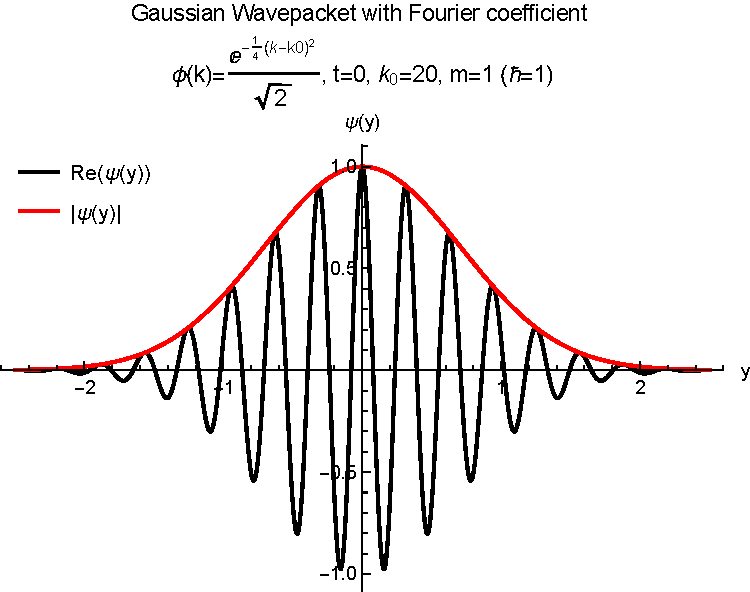
\includegraphics{plot4.pdf}
\caption{Gaussian wave packet (\ref{gauss1}) showing the carrier wave (black) and amplitude modulating envelope wave (red).}
\end{figure}

\noindent In this instance the integral in (\ref{gauss1}) can be accurately calculated by Taylor expansion of the dispersion relation around $k_0$ to first order. However this will not necessarily work for other plane waves, for example those in (\ref{wavefunction}). To make progress, one can use the stationary phase approximation; given Fourier coefficient $\phi(k)$ sharply localised around $k=k_0$, the integral (cf. (\ref{gauss1})) has non-zero value by dint of contributions from the integrand only in the region $k\approx k_0$, only if the plane wave term oscillates on scales larger than the region around $k_0$ (the wave phase is `stationary' in $k-$space). 

\noindent Applying this method to the incident and transmitted plane waves in (\ref{wavefunction}), (\ref{cont0}) (accounting for time evolution under the time evolution operator $U(t)=e^{-iEt/\hbar}$) yields:

\begin{subequations}
\begin{flalign}
	&\text{Incident:} && -\frac{1}{\hbar}\frac{dE}{dk}t+y_p(t)=0 \label{incidentpeak}&\\
	\intertext{from which one derives the group velocity of the wave packet $v_g = \hbar^{-1} dE/dk = \hbar k/m$. This is the propagation velocity of the envelope wave and is identified with the particle velocity. This differs from the phase velocity $v_p = w/k$ which is the propagation velocity of the carrier wave.}
	&\text{Transmitted:} && \frac{d\Delta\phi}{dk}-\frac{1}{\hbar}\frac{dE}{dk}t+y_p(t)-d=0 \label{transmittedpeak}
\end{flalign}
\end{subequations}

\noindent (cf. Hauge and St{\o}vneng 1989 (2.3)). Solving equations (\ref{incidentpeak}) and (\ref{transmittedpeak}) for $t$ at $y_p(t) = d/2 \text{ and } d/2$ respectively, one finds that the difference of these times, i.e. the traversal time of the peak across the barrier for the transmitted wave, is:

\begin{equation}
	\tau_\phi = \hbar \frac{d\Delta\phi}{dE} = \frac{m}{\hbar k}\frac{d\Delta\phi}{dk}
	\label{buttikerphasetime}
\end{equation}

\noindent (An identical result is obtained for a wave packet reflected from the barrier.) (cf. B{\"u}ttiker 1983 (3.1)).

Equation (\ref{buttikerphasetime}) can be calculated explicitly using equation (\ref{phasechange}):
\begin{subequations}
\begin{align}
	\frac{m}{\hbar k}\frac{d\Delta\phi}{dk}&=\frac{m}{\hbar k}\frac{d}{dk}\left(\arctan{\left[\frac{k^2-\kappa^2}{2k\kappa}\tanh{\kappa d}\right]}\right) \\
					       &=\frac{m}{\hbar k}\frac{1}{\left[\frac{k^2-\kappa^2}{2k\kappa}\tanh{\kappa d}\right]^2+1}\frac{1}{2}\frac{d}{dk}\left(\frac{k^2-\kappa^2}{k\kappa}\tanh{\kappa d}\right). \\ \intertext{Recalling the relation between $k$ and $\kappa$ in (\ref{wavefunction}), the derivative term evaluates to:}
					       &\left[2\kappa^{-1}+\frac{k^2}{\kappa^3}+\frac{\kappa}{k^2}\right]\tanh{\kappa d} + d\left(-\frac{k^2}{\kappa^2}+1\right)\sech^2{\kappa d}.\\ \intertext{Hence}
	\frac{m}{\hbar k}\frac{d\Delta\phi}{dk}&=\frac{m}{2\hbar k}\frac{4k^2\kappa^2\sech^2{\kappa d}}{(k^2-\kappa^2)^2\tanh^2{\kappa d}+4k^2\kappa^2}\left\{\left[2\kappa^{-1}+\frac{k^2}{\kappa^3}+\frac{\kappa}{k^2}\right]\sinh{\kappa d}\cosh{\kappa d}-\frac{kd}{\kappa}\left(\frac{k}{\kappa}-\frac{\kappa}{k}\right)\right\}\\
					       &=\frac{2mk\kappa^2}{\hbar}\frac{1}{k_0^4\sinh^2{\kappa d}+4k^2\kappa^2}\left\{\left[2\kappa^{-1}+\frac{k^2}{\kappa^3}+\frac{\kappa}{k^2}\right]\frac{\sinh{2\kappa d}}{2}-\frac{kd}{\kappa}\left(\frac{k}{\kappa}-\frac{\kappa}{k}\right)\right\}. \\ \intertext{The term in \{\dots\} is easily shown to be:}
	\{\dots\} &= \frac{k_0^4}{k^2\kappa^3}\frac{\sinh{2\kappa d}}{2}+\frac{d}{\kappa}(\kappa^2-k^2) \text{ where } k_0^2 = k^2+\kappa^2\\ \intertext{yielding the final result:}
	\tau_\phi &= \frac{m}{\hbar k \kappa}\frac{2k^2\kappa d(\kappa^2-k^2)+k_0^4\sinh{2\kappa d}}{4k^2\kappa^2+k_0^4\sinh^2{\kappa d}}. \label{phasedelaytime}
\end{align}
\end{subequations}
\noindent This is defined as the \textit{phase-delay time} of the scattering process (cf. B{\"u}ttiker 1983 (3.2)).
The same result is achieved via a different approach by Hauge and St{\o}vneng (1989). They introduce an interval $(y_1, y_2)$ containing the barrier (i.e. $y_1<-d/2,y_2>d/2$) and using (\ref{incidentpeak}) and (\ref{transmittedpeak}) define (cf. Hauge and St{\o}vneng 1989 (2.4)) the spatial delay $\delta y_T$ as the change in phase induced by the barrier and corresponding temporal delay $\delta\tau_T$ for the transmitted wave packet:

\begin{equation}
	\delta y_T = \frac{d\Delta\phi}{dk}-d \quad \delta\tau_T=\frac{1}{v(k)} \left[\frac{d\Delta\phi}{dk}-d\right] \quad \text{where $v(k) = \frac{\hbar k}{m}$ is the group velocity;}
	\label{transmittedphaseshift}
\end{equation}

\noindent with analogous definitions for the reflected wave packet:

\begin{equation}
	\delta y_R = d-\frac{d\Delta\phi}{dk} \quad \delta\tau_R=-\frac{1}{v(k)} \left[d-\frac{d\Delta\phi}{dk}\right].
	\label{reflectedphaseshift}
\end{equation}

\noindent They subsequently define (cf. Hauge and St{\o}vneng 1989 (2.5, 2.6)) the total phase time for transmission:

\begin{equation}
	\tau_T(y_1,y_2;k) = \frac{1}{v(k)}[y_2-y_1+\delta y_T]
\end{equation}

\noindent and similarly the total phase time for reflection:

\begin{equation}
	\tau_R(y_1,y_2;k) = \frac{1}{v(k)}[-2y_1-\delta y_R]
\end{equation}

\noindent where the minus sign before the spatial delay is picked up due to the wave packet travelling in the opposite direction.

\noindent By linearly extrapolating the interval $(y_1,y_2) \rightarrow (-d/2,d/2)$, one defines the \textit{extrapolated phase times} (cf. Hauge and St{\o}vneng 1989 (2.7, 2.8)):

\begin{align}
	\Delta\tau_T(-\frac{d}{2},\frac{d}{2};k) &= \frac{1}{v(k)}[d+\delta y_T] \label{deltataut}\\
	\Delta\tau_R(-\frac{d}{2},\frac{d}{2};k) &= \frac{1}{v(k)}[d-\delta y_R] \label{deltataur}.
\end{align}

\noindent Substituting $\delta y_T, \delta y_R$ in equations (\ref{transmittedphaseshift}) and (\ref{reflectedphaseshift}) into (\ref{deltataut}), (\ref{deltataur}) recovers (\ref{buttikerphasetime}) with $\Delta \tau_T := \Delta \tau_T(-d/2,d/2;k) \newline = \Delta \tau_R = \tau_\phi$.

\subsection{Dwell Time}
\label{subsection:dwelltime}

The \textit{dwell time} $\tau_D$ is an expression of the average time spent by a particle in the barrier region, regardless of whether it it ultimately transmitted or reflected (Leavens and Aers 1990 pp. 59). Formally it is defined as the ratio of the average number of particles within the barrier region to the average number entering or leaving the barrier per unit time (quantified by the incident flux j) (B{\"u}ttiker 1983 (3.5)), (Leavens and Aers 1989 (1)):

\begin{equation}
	\tau_D = \frac{\int_{-d/2}^{d/2}dy\,|\psi(t,y)|^2}{j(t,y)}.
	\label{dwelltimedef}
\end{equation}

\noindent Evaluating this quantity for the wave function inside the barrier region (\ref{wavefunction}), (\ref{cont0}) yields:
\begin{subequations}
\begin{align}
	\psi &= \frac{\kappa +ik}{2\kappa} T^{1/2}e^{i(\Delta\phi-kd/2)}e^{\kappa(y-d/2)} + \frac{\kappa-ik}{2\kappa}T^{1/2}e^{i(\Delta\phi-kd/2)}e^{-\kappa(y-d/2)}\\
	|\psi|^2 &= \frac{\kappa^2+k^2}{4\kappa^2}T\left(e^{\kappa(2y-d)}+e^{-\kappa(2y-d)}\right)+\frac{T}{4\kappa^2}\left((\kappa+ik)^2+(\kappa-ik)^2\right) \\
	\int_{-d/2}^{d/2}\,dy|\psi(y)|^2&=\int_{-d/2}^{d/2}\,dy\frac{T}{4\kappa^2}\left[(\kappa^2+k^2)\left(e^{\kappa(2y-d)}+e^{-\kappa(2y-d)}\right)+(\kappa+ik)^2+(\kappa-ik)^2\right] \\
					&= \int_{-d/2}^{d/2}\,dy\frac{T}{4\kappa^2}\left[(\kappa^2+k^2)2\cosh{\kappa(2y-d)}+2(\kappa^2-k^2)\right] \\
		 &= \frac{T}{4\kappa^2}\left[\frac{k_0^2}{\kappa}\sinh{2\kappa d}+2(\kappa^2-k^2)d\right] \\ \intertext{then, using equation (\ref{transmissionprobability}) for $T$:}
		 &= \frac{k^2}{\kappa}\frac{2\kappa d(\kappa^2-k^2)+k_0^2\sinh{2\kappa d}}{4k^2\kappa^2+k_0^4\sinh^2{\kappa d}}\\ \intertext{and for the incident flux with $\psi(y) = e^{iky}$:
}
j &= -\frac{i\hbar}{2m}\left(\psi^{*}\frac{\partial\psi}{\partial y}-\psi \frac{\partial \psi^{*}}{\partial y}\right) \label{1dflux}\\ 
  &= -\frac{i\hbar}{2m}(2ik) = \frac{\hbar k}{m} = v(k) \\ \intertext{so that (cf. B{\"u}ttiker 1983 (3.6)):}
	\tau_D &= \frac{1}{v(k)}\frac{k^2}{\kappa}\frac{2\kappa d(\kappa^2-k^2)+k_0^2\sinh{2\kappa d}}{4k^2\kappa^2+k_0^4\sinh^2{\kappa d}}.
	\label{dwelltime}
\end{align}
\end{subequations}

\noindent The phase times $\tau_T \text{ and } \tau_R$ represent conditional averages over mutually exclusive events (a particle cannot both reflect and transmit) (Hauge and St{\o}vneng 1989 pp. 918). The dwell time $\tau_D$ is the average over all scattering channels, and hence the conditional averages must obey the probabilistic rule:

\begin{equation}
	\tau_D = T\tau_T+R\tau_R
	\label{dwellcondition}
\end{equation}

\noindent where $T \text{ and } R = 1-T$ are transmission and reflection probabilities respectively. Comparison of equations (\ref{phasedelaytime}) and (\ref{dwelltime}) show this consistency check is not satisfied:

\begin{equation}
	\tau_T = \tau_R = \tau_\phi \implies T\tau_T+R\tau_R = \tau_\phi(T+R) = \tau_\phi \neq \tau_D. 
\end{equation}

Resolution of this issue comes from noticing that attaching \textit{physical significance} to the time in (\ref{phasedelaytime}) is incorrect, as it requires the assumption that motion outside of the barrier is that of a free particle (Hauge and St{\o}vneng (1989 pp. 924)). This is valid on the transmitted side of the barrier, however during approach to the barrier the incoming wave packet interferes with the reflected wave packet and hence motion can no longer be assumed to be free.
\subsection{Continuous Cyclic Quantum Clock}
\label{subsection:ccqc}

In this section I present a theoretical model of a continuous cyclic quantum clock as provided by Hilgevoord (2002). This model acts as a precursor to the discrete cyclic quantum clock presented in section \ref{subsection:dcqc}.

The angular variable $\phi$ plays the role of the clock variable and is represented by the operator $\hat{\Phi}$. An angular momentum operator $\hat{L}$ is also introduced and the two operators in the angular representation are given by (setting $\hbar = 1$):

\begin{equation}
	\hat{\Phi} = \phi \quad \hat{L} = -i \frac{d}{d\phi}
\end{equation}

\noindent as is familiar from the theory of angular momentum in quantum mechanics. These operators act on a Hilbert space of square integrable functions of $\phi$ with domain $[0,2\pi]$ as:

\begin{equation}
	\hat{\Phi} f(\phi) = \phi f(\phi) \quad \hat{L} f(\phi) = -i \frac{d}{d\phi}f(\phi).
\end{equation}

\noindent These operators have eigenvalue equations 

\begin{equation}
	\hat{\Phi}\ket{\phi} = \phi\ket{\phi}, \phi \in [0,2\pi] \quad \hat{L}\ket{m} = m\ket{m}, m = 0, \pm 1, \pm 2,\dots
\end{equation}

\noindent in which the eigenvectors form complete orthonormal sets such that:

\begin{equation}
	\braket{\phi|\phi'} = \delta(\phi-\phi ') \quad \braket{m|m'} = \delta_{mm'}.
\end{equation}

\noindent Recalling from the theory of angular momentum in quantum mechanics that the $\hat{L}_z = -i \frac{d}{d\phi}$ operator has eigenfunctions $\propto e^{im\phi}$, $\ket{m}$ has wave function $\braket{\phi|m}= Ae^{im\phi}$ where $A$ is calculated using the normalisation condition to be $(2\pi)^{-\frac{1}{2}}$:

\begin{equation}
	u_m(\phi) := \braket{\phi|m} = (2\pi)^{-\frac{1}{2}}e^{im\phi}.
\end{equation}

\noindent As $\{\ket{m}\}$ form a complex set, $\ket{\phi}$ can be expressed as:

\begin{equation}
	\ket{\phi} = (2\pi)^{-\frac{1}{2}}\sum_{m=-\infty}^{\infty}e^{-im\phi}\ket{m}.
	\label{phiexpansion}
\end{equation}

\noindent Introducing the Hamiltonian $\hat{H}=\omega \hat{L}$, the time evolution operator $U(t) = e^{-iHt}$ acts as:

\begin{subequations}
\begin{align}
\hat{L}e^{-im\phi}\ket{m} &= e^{-im\phi}\hat{L}\ket{m} \text{ by linearity of } \hat{L} \\
				  &= me^{-im\phi}\ket{m} \\
\implies e^{-iHt}\ket{\phi} &= \sum_{n=0}^{\infty}\frac{(-i\omega t)}{n!}^n \hat{L}^n \left((2\pi)^{-\frac{1}{2}}\sum_{m=-\infty}^{\infty}e^{-im\phi}\ket{m}\right) \\
			   &= (2\pi)^{-\frac{1}{2}}\sum_{n=0}^{\infty}\sum_{m=-\infty}^{\infty} \frac{(-i\omega mt)}{n!}^n e^{-im\phi} \ket{m} \\
				   &= (2\pi)^{-\frac{1}{2}}\sum_{m=-\infty}^{\infty}e^{-i\omega mt}e^{-im\phi}\ket{m} \\
				   &= \ket{\phi+\omega t}
\end{align}
\end{subequations}
\noindent by setting $\omega = 1, \space \phi$ plays exactly the same role as a time variable $t$.

\subsection{Discrete Cyclic Quantum Clock}
\label{subsection:dcqc}
A discrete cyclic quantum clock can be modelled by limiting the sum in equation (\ref{phiexpansion}) to values of \linebreak $m \text{ satisfying } -j \leq m \leq j$, as presented by Peres (1980). The clock has an odd number $N = 2j+1$ of states represented by wave functions

\begin{equation}
	u_m(\phi) = (2\pi)^{-\frac{1}{2}}e^{im\phi}, m = -j,\dots, j \text{ and } 0 \leq \phi \leq 2\pi.
\end{equation}

\noindent One can construct an alternative orthogonal basis for the clock's wave functions
\begin{subequations}
\begin{align}
	v_k(\phi) &= N^{-\frac{1}{2}}\sum_{m=-j}^j e^{-2\pi ikm/N}u_m \label{vkexpansion}\\
		    &= (2\pi N)^{-\frac{1}{2}}\sum_{m=-j}^j [e^{i(\phi-2\pi k/N)}]^m \quad \tilde{m} = m+j \\
		    &= (2\pi N)^{-\frac{1}{2}}\sum_{\tilde{m}=0}^{2j} [e^{i(\phi-2\pi k/N)}]^{\tilde{m}-j} \\
		    &= (2\pi N)^{-\frac{1}{2}}[e^{i(\phi-2\pi k/N)}]^{(1-N)/2}\sum_{\tilde{m}=0}^{2j}[e^{i(\phi-2\pi k/N)}]^{\tilde{m}} \\
		    &= (2\pi N)^{-\frac{1}{2}}[e^{i(\phi-2\pi k/N)}]^{(1-N)/2}\left(\frac{1-(e^{i(\phi-2\pi k/N)})^N}{1-e^{i(\phi-2\pi k/N)}}\right) \\
		    &= (2\pi N)^{-\frac{1}{2}}\frac{\sin{\frac{N}{2}(\phi-2\pi k/N)}}{\sin{\frac{1}{2}(\phi-2\pi k/N)}} \text{ for } k = 0,\dots,N-1.
\end{align}
\end{subequations}

\noindent For large $N$ these functions have a sharp peak at $\phi = 2\pi k/N$ (see Figure \ref{fig:wavepeak}), which we visualise as pointing to the $k^{th}$ hour with angle uncertainty $\pm \pi/N$:

\begin{figure}[ht]
\centering
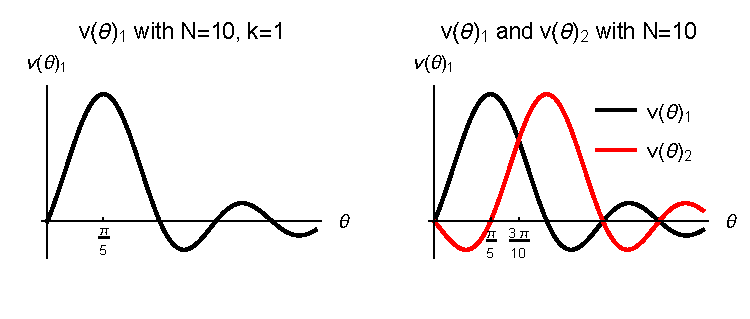
\includegraphics{plot1.pdf}
\caption{The wave functions of the discrete cyclic quantum clock are sharply peaked around $\phi = 2\pi k/N$}
\label{fig:wavepeak}
\end{figure}

\noindent One can then define projection operators $P_kv_m=\delta_{km}v_m$ and a clock time operator $T_c = \tau\sum{kP_k}$ where $\tau$ is the resolution of the clock. The eigenvectors of $T_c$ are $v_k$ with eigenvalues $t_k = k\tau, k=0,\dots,N-1$. Hence measuring $T_c$ yields discrete approximations to the true time, just as analog and digital clocks do. 

\noindent The clock's Hamiltonian is:

\begin{equation}
	H_c = \omega J \text{ where } \omega = \frac{2\pi}{N\tau} \text{ and } J=-i\hbar \frac{\partial}{\partial\phi}
	\label{clockhamiltonian}
\end{equation}

\noindent The wave functions $u_m$ are eigenfunctions of the Hamiltonian:

\begin{equation}
	H_cu_m = m\hbar\omega u_m;
	\label{clockwavefunctions}
\end{equation}

\noindent whence expanding the time evolution operator as a Taylor series gives:
\begin{subequations}
\begin{align}
	e^{-iH_ct/\hbar}u_m &= e^{-im\omega t}u_m = (2\pi)^{-\frac{1}{2}}e^{im(\theta-\phi t)} \\
	\implies e^{-iH_c\tau/\hbar}v_k &= N^{-\frac{1}{2}}\sum_{m}e^{-2\pi ikm/N}e^{-2\pi im/N}u_m \\
						       &= N^{-\frac{1}{2}}\sum_{m}e^{-2\pi im(k+1)/N}u_m \\
						       &= v_{k+1}.
\end{align}
\end{subequations}

\subsubsection{Application: Timing an Atomic Decay}
One can apply the construction of the quantum clock to model timing an atomic decay (Peres 1980 section 4). The atom-clock system has Hamiltonian $H=H_a+P_0H_c$ where $H_a$ is the Hamiltonian of the atom, $H_c$ the Hamiltonian of the clock and $P_0$ the projection operator for the atom's undecayed state. This coupling therefore represents the notion that the clock stops running when the atom decays. $H_a$ is of the form $H_a=H_0+V$ where $H_0$ has a continuous spectrum $H_0\phi(E) = E\phi(E) \quad E>E_{min}$, plus one discrete eigenstate $\phi_0$ with energy $E_0>E_{min}$. The non vanishing matrix elements of $V$ are denoted $V(E) := \braket{\phi(E)|V|\phi_0}$, which is assumed to be almost constant in $E$ over a large domain on both sides of $E_0$. In sum, one has:

\begin{equation}
	H=H_a+P_0H_c=H_0+V+P_0H_c.
\end{equation}

The wave function for the atom can be expressed as:

\begin{equation}
	\psi = a_0\phi_0e^{-iE_0t/\hbar}+\int dE\, a(E)\phi(E)e^{-iEt/\hbar}.
\end{equation}

\noindent Application of the Schr{\"o}dinger equation for the atom yields:

\begin{equation}
	i\hbar \dot{a}(E) = V(E)a_0e^{i(E-E_0)t/\hbar}.
	\label{aODE}
\end{equation}


\begin{proof}
\begin{subequations}
\begin{align}
	\ket{\psi} &= a_0\ket{\phi_0}e^{-iE_0t/\hbar}+\int dE\,a(E)\ket{\phi(E)}e^{-iEt/\hbar} \\
	\implies (H_0+V)\ket{\psi} &= a_0E_0\ket{\phi_0}e^{-iE_0t/\hbar}+\int dE\, a(E)E\ket{\phi(E)}e^{-iEt/\hbar} \\ 
				   &+a_0V\ket{\phi_0}e^{-iE_0t/\hbar}+\int dE\, a(E)V\ket{\phi(E)}e^{-iEt/\hbar} \nonumber\\
				   &= i\hbar \frac{d\ket{\psi}}{dt}.
\end{align}
\end{subequations}

\noindent Taking the inner product with $\bra{\phi(E')}$ on both sides and using the orthogonality conditions yields the final result.
\end{proof}
\noindent $a_0$ is given by the Weisskopf-Wigner ansatz, i.e. $a_0 = e^{-\gamma t/\hbar}$. Substitution into (\ref{aODE}) and taking the limit as $t \rightarrow \infty$ yields:

\begin{equation}
	\lim_{t\to\infty}a(E) = \frac{V(E)}{E-E_0+i\gamma}
\end{equation}

\noindent and 

\begin{equation}
	\lim_{t\to\infty}\psi(t) = \int dE\,\frac{V(E)\phi(E)e^{-iEt/\hbar}}{E-E_0+i\gamma}.
\end{equation}

\noindent Normalisation of the wave function implies:

\begin{equation}
	\int dE\,\frac{|V(E)|^2}{(E-E_0)^2+\gamma^2}=1
	\label{atomdecaynormalisation}
\end{equation}

\noindent Using the identity:

\begin{equation}
	\delta(E-E_0) = \frac{1}{\pi} \lim_{\gamma\to 0}\frac{\gamma}{(E-E_0)^2+\gamma^2} \approx \frac{\gamma}{\pi} \frac{1}{(E-E_0)^2+\gamma^2}
\end{equation}

\noindent in (\ref{atomdecaynormalisation}) yields $\gamma = \pi|V(E_0)|^2$.

\noindent Coupling the atom to a clock using the clock Hamiltonian in (\ref{clockhamiltonian}):

\begin{equation}
	H = H_a+P_0\omega J
\end{equation}

\noindent and setting the initial state of the clock to $v_0 = 1/\sqrt{N}\sum u_n$ as in (\ref{vkexpansion}), $J$ can be replaced by the numerical constant $n\hbar$ by virtue of the eigenvalue equation (\ref{clockwavefunctions}). Note this shifts the energy of the initial state $E_0 \rightarrow E_0 + n\hbar\omega$.

\noindent In the limit of large $t$ the combined state of the atom and clock is:

\begin{equation}
	\psi = N^{-\frac{1}{2}}\sum u_n \int dE \, \frac{V(E)\phi(E)e^{-iEt/\hbar}}{E-E_0-n\hbar\omega+i\gamma}.
\end{equation}

\noindent The density matrix representing the state of the clock is given by (Peres 1980 pp. 555):

\begin{equation}
	\rho = Tr_a(\ket{\psi}\bra{\psi}) = \frac{1}{N}\sum \frac{\ket{u_n}\bra{u_m}}{1+i\alpha(n-m)}
\end{equation}

\noindent where $Tr_a$ indicates the trace is to be taken over the atom degrees of freedom only, and $\alpha = \hbar\omega/2\gamma$ is the angle through which the pointer turns during an average atom lifetime $\hbar/2\gamma$. From this the probability $\langle P_k \rangle$ of finding the clock stopped at time $t_k = k\tau \stackrel{(\ref{clockhamiltonian})}{=} 2\pi k/N\omega$ is given by:
\begin{subequations}
\begin{align}
	Tr(\rho P_k) &= \frac{1}{N}\sum_{m,n} \frac{\braket{v_k|u_n}\braket{u_m|v_k}}{1+i\alpha(n-m)} \\
		     &\stackrel{\mathclap{(\ref{vkexpansion})}}{=} \frac{1}{N^2}\sum_{m,n=-j}^j \frac{e^{2\pi ik(n-m)/N}}{1+i\alpha(n-m)}.
\end{align}
\end{subequations}

\noindent The double summation can be evaluated as follows: Let $p=n-m \text{ and } q=n+m$. The summation becomes:

\begin{equation}
	Tr(\rho P_k) = \frac{1}{N^2}\sum_{p=-2j}^{2j}\sum_{q=q_1(p)}^{q_2(p)}\frac{e^{i\theta p}}{1+i\alpha p}
\end{equation}

\noindent where $\theta = 2\pi k/N, q_1 \text{ and } q_2$ are bounds that can be determined as follows:

\begin{figure}[ht]
    \centering
    \incfig{doublesumdiagram}
    \caption{Bounds of the double sum in $p,q$ coordinates}
    \label{fig:doublesumdiagram}
\end{figure}

\noindent For fixed $p \in \{-2j,-2j+1,\dots,2j-1,2j\}$, demonstrated by the dashed line in Figure \ref{fig:doublesumdiagram}, the upper and lower bounds can be read off to be:

\begin{equation}
	q_1(p)=-2j+|p| \quad q_2(p)=2j-|p|
\end{equation}

\noindent Next noting that for fixed $p$ of given parity, all $q \in \{q_1(p),\dots,q_2(p)\}$ have the same parity and hence:

\begin{subequations}
\begin{align}
	Tr(\rho P_k) &= \frac{1}{N^2}\sum_{p=-2j}^{2j}\frac{e^{i\theta p}}{1+i\alpha p}\sum_{q=-2j+|p|}^{2j-|p|}1 \\
		     &= \frac{1}{N^2}\sum_{p=-2j}^{2j}\frac{e^{i\theta p}}{1+i\alpha p}\left[\frac{2j-|p|-(-2j+|p|)}{2}+1\right] \\
		     &= \frac{1}{N^2}\sum_{p=-2j}^{2j}\frac{(N-|p|)e^{i\theta p}}{1+i\alpha p} \approx \frac{1}{N}\sum_{p=-2j}^{2j}\frac{e^{i\theta p}}{1+i\alpha p}
\end{align}
\end{subequations}

\noindent This result can be recognised as the Fourier series expansion of $\frac{2\pi e^{-\theta/\alpha}}{N\alpha\left(1-e^{-2\pi/\alpha}\right)}$; and hence the clock stops (atoms decay) according to the exponential decay law, as expected.

\subsection{Larmor Precession}
\label{subsection:larmorprecession}
In this section I consider the quantum barrier experiment as in section \ref{subsection:quantumbarrier}, but now with the additional constraints that the particles carry spin $s=1/2$ polarised in the x-direction, and with the presence of a small magnetic field $\boldsymbol{B_0}$ parallel with the z-axis and confined to the width of the barrier (see Figure \ref{fig:potentialbarrierfield}) (B{\"u}ttiker 1983 section 1).

\begin{figure}[ht]
    \centering
    \incfig{potentialbarrierplusfield}
    \caption{Experimental set up of a quantum barrier with a magnetic field constrained inside.}
    \label{fig:potentialbarrierfield}
\end{figure}

\noindent The magnetic field engenders on the particles in the barrier a Larmor precession of frequency $\omega_L = g\mu B_0/\hbar$, where $g$ is the gyromagnetic ratio and $\mu$ is the magnetic moment. This changes the spin of the particles to be polarised in the x-y plane such that:

\begin{equation}
	\langle S_x \rangle \approx \frac{\hbar}{2} \quad \langle S_y \rangle \approx -\frac{\hbar}{2}\omega_L\tau_y.
\end{equation}

\noindent The presence of the magnetic field and barrier also induces a component of spin in the z-direction, although through an alternative mechanism: Recall from the theory of spin in quantum mechanics that particles with spin in the x-direction can be represented as a linear combination of particles in the $\pm \text{z}$ direction:

\begin{equation}
	\ket{x; \pm} = \frac{1}{\sqrt{2}}\ket{z;+} \pm \frac{1}{\sqrt{2}}\ket{z;-}
\end{equation}

\noindent with z-components $\pm \hbar/2$ each with probability 0.5. Inside the barrier the magnetic field induces a Zeeman shift $\pm \hbar\omega_L/2$ to the energies of the particles, giving rise to different exponential decays of the wave functions inside the barrier (\ref{wavefunction})\footnote{Note I ignore the exponentially growing term in (\ref{wavefunction}) because it is multiplied by a suppressive pre-factor $e^{-\kappa d/2}$ in equation (\ref{cont0}).} (cf. B{\"u}ttiker 1983 (1.5)):

\begin{equation}
	\kappa_{\pm}=(k_0^2-k^2\mp \frac{m\omega_L}{\hbar})^{\frac{1}{2}}
\end{equation}

\noindent where $\kappa_{+}(\kappa_{-})$ corresponds to particles with spin z parallel(antiparallel) to the magnetic field.

\noindent In the limit $\boldsymbol{B_0} \propto \omega_L \text{ is small}, \kappa_{\pm}$ can be approximated as:
\begin{subequations}
\begin{align}
   \kappa_{\pm} &= \left(k^{2}_{0}-k^{2} \mp \frac{m \omega_{L}}{\hbar}\right)^{\frac{1}{2}}\\	
		&= \kappa \left(1 \mp \frac{m \omega_{L}}{\hbar \kappa^{2}}\right)^{\frac{1}{2}}\\
		&\approx \kappa \left(1 \mp \frac{m \omega_{L}}{2\hbar \kappa^{2}}\right)\\
		&= \kappa \mp \frac{m \omega_{L}}{2\hbar \kappa} \label{smallfieldkappa}.
\end{align}
\end{subequations}

\noindent As $\kappa_{+} < \kappa_{-}$, particles with spin aligned with the magnetic field penetrate more easily than particles with spin anti-aligned with the field, reflected in the transmission probability (cf. B{\"u}ttiker 1983 (1.7)):

\begin{align}
	T &\stackrel{\mathclap{(\ref{transmissionprobability})}}{=} \left[1+\frac{(k^2+\kappa^2)^2\sinh^2{\kappa d}}{4k^2\kappa^2}\right]^{-1}\\
	  &\approx \left[\frac{(k^2+\kappa^2)^2}{4k^2\kappa^2}\frac{e^{2\kappa d}}{4}\right]^{-1} \\
	&= \frac{16k^2\kappa^2}{k^2+\kappa^2}e^{-2\kappa d} \\
	\implies T_{\pm} &= Te^{\pm\omega_L \tau_z} 
\end{align}

\noindent where $\tau_z = md/\hbar\kappa$ is the time a particle with velocity $v(k) = \hbar k/m$ takes to traverse the barrier (the subscript `$z$' is chosen because the quantity arises in the spin-z expectation value (\ref{eqn:sz}), and does not denote the propagation ($y$) direction). Hence the barrier with the magnetic field induces a net $z$-component of spin polarisation aligned with the field, quantified the ratio of excess flux to total flux:

\begin{equation}
	\langle S_z \rangle = \frac{\hbar}{2}\frac{T_{+}-T_{-}}{T_{+}+T_{-}} = \frac{\hbar}{2}\tanh{\omega_L\tau_z}.
	\label{eqn:sz}
\end{equation}

\noindent The polarisation of the transmitted and reflected particles for all incident energies can be calculated. To do so one must solve the scattering problem with the Hamiltonian (cf. B{\"u}ttiker 1983 (2.1)):

\begin{equation}
	H = 
	\begin{cases}
	\left(\frac{p^2}{2m} + V_0\right)\mathbb{1}-\left(\frac{\hbar \omega_L}{2}\right) \sigma_z & |y| \leq \frac{d}{2}\\
	\left(\frac{p^2}{2m}\right)\mathbb{1} & |y| \geq \frac{d}{2}
	\end{cases}
	\end{equation}
where $\mathbb{1}$ is the $2 \times 2$ identity matrix and $\sigma_{x}, \sigma_{y}, \sigma_{z}$ are the Pauli spin matrices.

\noindent $H$ acts on spinors
\begin{align}
	\psi &= \begin{pmatrix}
		\psi_{+}(y) \\
		\psi_{-}(y)
		\end{pmatrix}.
\end{align}

As usual $|\psi_{\pm}(y)|^{2}dy$ is the probability of finding a particle \textit{upon measurement} with spin $\pm \hbar/2$ in the interval $y, y+dy$. I emphasise `upon measurement' here as this is an important point of distinction between the orthodox and pilot-wave interpretations addressed in this essay. The incident beam is polarised in the $x$-direction:
\begin{align}
	\psi = \frac{1}{\sqrt{2}}
	\begin{pmatrix}
	1\\
	1
	\end{pmatrix}
	e^{iky}
\end{align}
i.e. $\psi$ is an eigenvector of $S_{x}$.

\noindent $H$ is diagonal in the spinor basis so one can solve the scattering problem for particles with spin $\hbar/2$ and $-\hbar/2$ separately. This amounts to solving the quantum barrier in (\ref{wavefunction}) with the following adjustments:

For particles with spin aligned(anti-aligned) with the magnetic field:

\begin{itemize}
	\item $\kappa \to \kappa_{+}(\kappa_{-})$
	\item $V_0 \to V_0+(-)\frac{\hbar \omega_L}{2}$
	\item $A,B,C,D \text{ in } (\ref{cont0}) \to A_{+(-)},B_{+(-)},C_{+(-)},D_{+(-)} \text{ by replacing } \kappa \to \kappa_{+}(\kappa_{-})$.
\end{itemize}

\subsubsection{The Strong-Field Limit}
The transmitted particles have spinor:

\begin{equation}
	\psi_T = (|D_{+}|^2+|D_{-}|^2)
	\begin{pmatrix}
		D_{+}\\
		D_{-}\\
	\end{pmatrix}.
\end{equation}

\noindent Recalling the Pauli sigma matrices:
\begin{equation}
	\sigma_x = 
	\begin{pmatrix}
		0&1\\
		1&0
	\end{pmatrix} \quad
	\sigma_y = 
	\begin{pmatrix}
		0&-i\\
		i&0
	\end{pmatrix} \quad
	\sigma_z =
	\begin{pmatrix}
		1&0\\
		0&-1
	\end{pmatrix}
\end{equation}

\noindent one finds for the expectation values of spin for the transmitted particles (cf. B{\"u}ttiker 1983 (2.11)):
\begin{subequations}
\begin{align}
	\langle S_z \rangle_T &= \frac{\hbar}{2}\braket{\psi_T|\sigma_z|\psi_T}=\frac{\hbar}{2}\frac{|D_+|^2+|D_-|^2}{|D_+|^2+|D_-|^2} \\
	\langle S_y \rangle_T &= \frac{\hbar}{2}\braket{\psi_T|\sigma_y|\psi_T}=i\frac{\hbar}{2}\frac{D_+D_-^*-D_+^*D_-}{|D_+|^2+|D_-|^2} \\
	\langle S_x \rangle_T &= \frac{\hbar}{2}\braket{\psi_T|\sigma_x|\psi_T}=\frac{\hbar}{2}\frac{D_+D_-^*+D_+^*D_-}{|D_+|^2+|D_-|^2}.
\end{align}
\end{subequations}

\noindent Using (\ref{cont0}) and the adjustments for the magnetic field outlined above, one finds (cf. B{\"u}ttiker 1983 (2.12a-c)):

\begin{equation}
	\langle S_z \rangle_T = \frac{\hbar}{2}\frac{T_+-T_-}{T_++T_-}.
	\label{szT}
\end{equation}


\begin{proof}
Follows immediately from the fact that $T=|D|^2$.
\end{proof}

\begin{equation}
	\langle S_y \rangle_T = -\hbar \sin{(\Delta\phi_+-\Delta\phi_-)}\frac{(T_+T_-)^{\frac{1}{2}}}{T_++T_-}.
	\label{syT}
\end{equation}

\begin{proof}
\begin{subequations}
\begin{align}
	\langle S_y \rangle_T &= i\frac{\hbar}{2}\left(\frac{(T_+T_-)^{\frac{1}{2}}}{T_++T_-}\right)\left(e^{i(\Delta\phi_+-\Delta\phi_-)}-e^{-i(\Delta\phi_+-\Delta\phi_-)}\right) \\
			    &= i\frac{\hbar}{2}\left(\frac{(T_+T_-)^{\frac{1}{2}}}{T_++T_-}\right)(2i\sin{(\Delta\phi_+-\Delta\phi_-)}) \\
			    &=-\hbar \sin{(\Delta\phi_+-\Delta\phi_-)}\frac{(T_+T_-)^{\frac{1}{2}}}{T_++T_-}.
\end{align}
\end{subequations}
\end{proof}

\begin{equation}
	\langle S_x \rangle_T = \hbar \cos{(\Delta\phi_+-\Delta\phi_-)}\frac{(T_+T_-)^{\frac{1}{2}}}{T_++T_-}
	\label{sxT}
\end{equation}

\noindent follows along similar lines to the case of $\langle S_y \rangle_T$.

\noindent These derivations have used no assumptions about the strength of the field, and so they hold for arbitrary magnetic field. Using (\ref{transmissionprobability}) one sees that $T_+ \propto e^{-2\kappa_+d} \text{ and } T_- \propto e^{-2\kappa_-d}$. As $\kappa_- > \kappa_+$, for a sufficiently opaque barrier ($k_0d \gg 1$), $T_+ \gg T_-$, and therefore:

\begin{equation}
	\langle S_z \rangle_T \approx \frac{\hbar}{2} \quad \langle S_y \rangle_T = \langle S_x \rangle_T \approx 0.
\end{equation}

\noindent Hence the transmitted beam is almost exclusively polarised parallel to the magnetic field.

\noindent By similar arguments, with the spinor:

\begin{equation}
	\psi_R = (|A_{+}|^2+|A_{-}|^2)
	\begin{pmatrix}
		A_{+}\\
		A_{-}\\
	\end{pmatrix}
\end{equation}

\noindent one arrives at the analogous results for the reflected wave (cf. B{\"u}ttiker 1983 (2.14)):
\begin{subequations}
\begin{align}
	\langle S_z \rangle_R &= \frac{\hbar}{2}\frac{R_+-R_-}{R_++R_-}\\
	\langle S_y \rangle_R &= -\hbar \sin{(\Delta\phi_+-\Delta\phi_-)}\frac{(R_+R_-)^{\frac{1}{2}}}{R_++R_-}\\
	\langle S_x \rangle_R &= \hbar \cos{(\Delta\phi_+-\Delta\phi_-)}\frac{(R_+R_-)^{\frac{1}{2}}}{R_++R_-}.
\end{align}
\end{subequations}
\noindent Using the statement of particle conservation $R_+-R_-=-(T_+-T_-)$, one finds that:

\begin{subequations}
\label{stsrrelations}
\begin{align}
	\langle S_z \rangle_R &= -\langle S_z \rangle_T \frac{T_++T_-}{R_++R_-}\\
	\langle S_y \rangle_R &= \langle S_y \rangle_T \left(\frac{R_+R_-}{T_+T_-}\right)^{\frac{1}{2}}\frac{T_++T_-}{R_++R_-} \\
	\langle S_x \rangle_R &= \langle S_x \rangle_T \left(\frac{R_+R_-}{T_+T_-}\right)^{\frac{1}{2}}\frac{T_++T_-}{R_++R_-}
\end{align}
\end{subequations}

\noindent and hence $\langle S_z \rangle_R + \langle S_z \rangle_T = 0$, the statement of conservation of angular momentum. 

\subsubsection{Infinitesimal Field}
In this section I report the study of polarisation of the transmitted and reflected waves in the limit of an infinitesimal field. Using (\ref{smallfieldkappa}), one finds the result (cf. B{\"u}ttiker 1983 (2.16)):

\begin{subequations}
\begin{align}
	T_+-T_- &= T(\kappa_+)-T(\kappa_-)\\
		&= \frac{T(k-m\omega_L/2\hbar\kappa)-T(k+m\omega_L/2\hbar\kappa)}{m\omega_L/\hbar\kappa}\times \frac{m\omega_L}{\hbar\kappa} \\
		&\approx-\left(\frac{m\omega_L}{\hbar\kappa}\right)\frac{\partial T}{\partial \kappa}. \label{netT}
\end{align}
\end{subequations}

\noindent In equation (\ref{netT}) the Larmor frequency $\omega_L$ is multiplied by a time $(m/\hbar\kappa) \partial T/\partial \kappa$. This motivates the definition of the characteristic times $\tau_{zT}, \tau_{yT}, \tau_{xT}$ such that:

\begin{subequations}  
\label{characteristictransmissiontimes}
\begin{align}	
	\langle S_z \rangle_T &= \frac{\hbar}{2}\omega_L\tau_{zT} \\
	\langle S_y \rangle_T &= -\frac{\hbar}{2}\omega_L\tau_{yT} \\
	\langle S_x \rangle_T &= \frac{\hbar}{2}\left(1-\frac{\omega_L^2\tau_{xT}^2}{2}\right).
\end{align}
\end{subequations}

\noindent Using equations (\ref{szT}), (\ref{syT}) and (\ref{sxT}) and the approximation $T_++T_- \approx 2T$, one can derive explicit results for the characteristic times (cf. B{\"u}ttiker 1983 (2.18a-c)):

\begin{equation}
	\tau_{zT} = -\left(\frac{m}{\hbar\kappa}\right)\frac{\partial \ln{T^{\frac{1}{2}}}}{\partial\kappa}. \label{tauz}
\end{equation}

\begin{proof}
\begin{subequations}
\begin{align}
	\langle S_z \rangle_T &\stackrel{\mathclap{(\ref{szT})}}{=}\,\frac{\hbar}{2}\frac{T_+-T_-}{T_++T_-}\\
	&\approx \frac{\hbar}{4}\frac{T_+-T_-}{T}\\
	&\stackrel{\mathclap{(\ref{netT})}}{=}\,-\frac{m\omega_L}{\hbar\kappa}\frac{\hbar}{4}\frac{1}{T}\frac{\partial T}{\partial \kappa} \\
	&=-\frac{m\omega_L}{\hbar\kappa}\frac{\hbar}{2}\frac{\partial\ln{T^{\frac{1}{2}}}}{d\kappa} \\
	&=\frac{\hbar}{2}\omega_L\tau_{zT}.
\end{align}
\end{subequations}
\end{proof}

\begin{equation}
	\tau_{yT} = -\left(\frac{m}{\hbar\kappa}\right)\frac{\partial\Delta\phi}{\partial\kappa}. \label{tauy}
\end{equation}

\begin{proof}
\begin{subequations}
\begin{align}
	\langle S_y \rangle_T &\stackrel{\mathclap{(\ref{syT})}}{=}\,-\hbar \sin{(\Delta\phi_+-\Delta\phi_-)}\frac{(T_+T_-)^{\frac{1}{2}}}{T_++T_-}\\
	\sin{(\Delta\phi_+-\Delta\phi_-)} &\approx \Delta\phi_+-\Delta\phi_- \approx \Delta(\Delta\phi) \text{ where } \Delta\phi := \phi_+-\phi_-\\
	\implies \langle S_y \rangle_T &\approx -\frac{\hbar}{2}\Delta(\Delta\phi) \text{ as } \frac{(T_+T_-)^{\frac{1}{2}}}{T_++T_-} \approx \frac{1}{2} \\
	\Delta\kappa &:= \kappa_+-\kappa_- = -\frac{m\omega_L}{\hbar\kappa} \\
\implies \langle S_y \rangle_T &= -\frac{\partial\Delta\phi}{\partial\kappa}\left(\frac{m\omega_L}{\hbar\kappa}\right) \\
			       &=-\frac{\hbar}{2}\omega_L\tau_{yT}.
\end{align}
\end{subequations}
\end{proof}

\begin{subequations}\label{taux}
\begin{align}
	\tau_{xT} &= \left(\frac{m}{\hbar\kappa}\right)\left[\left(\frac{\partial\Delta\phi}{\partial\kappa}\right)^2+\left(\frac{\partial\ln{T^{\frac{1}{2}}}}{\partial\kappa}\right)^2\right]^{\frac{1}{2}}\label{tauxpart1} \\
	       &=\left(\frac{m}{\hbar\kappa}\right)\left|D^{-1}\frac{\partial D}{\partial\kappa}\right|. \label{tauxpart2}
\end{align}
\end{subequations}

\begin{proof} Equation (\ref{tauxpart1}) can be proven using similar methods to above but can be proven more easily by noting that since $\langle S_x \rangle^2 + \langle S_y \rangle^2 + \langle S_z \rangle^2 = \frac{\hbar^2}{4}$ then $\tau_{xT} = (\tau_{yT}^2+\tau_{zT}^2)^\frac{1}{2}$. Equation (\ref{tauxpart2}) follows simply using the form of $D$ in (\ref{cont0}).
\end{proof}

\noindent The derivatives in (\ref{tauz}), (\ref{tauy}) can be evaluated explicitly to give:

\begin{equation}
	\tau_{zT} = \frac{mk_0^2}{\hbar\kappa^2}\frac{(\kappa^2-k^2)\sinh^2{\kappa d}+\left(\frac{\kappa d k_0^2}{2}\right)\sinh{2\kappa d}}{4k^2\kappa^2+k_0^4\sinh^2{\kappa d}}.
\end{equation}

\begin{proof}
\begin{subequations}
\begin{align}
	\tau_{zT} &\stackrel{\mathclap{(\ref{tauz})}}{=} -\left(\frac{m}{\hbar\kappa}\right)\frac{\partial \ln{T^{\frac{1}{2}}}}{\partial\kappa} \\
	\ln{T^{\frac{1}{2}}}&=\frac{m}{2\hbar\kappa}\frac{\partial}{\partial\kappa}\ln{\left[1+\frac{(k^2+\kappa^2)^2\sinh^2{\kappa d}}{4k^2\kappa^2}\right]} \\
			    &=\frac{m}{2\hbar\kappa}\left[1+\frac{k_0^4\sinh^2{\kappa d}}{4k^2\kappa^2}\right]^{-1}\frac{1}{4k^2}\frac{\partial}{\partial\kappa}\left[\frac{k_0^4\sinh^2{\kappa d}}{\kappa^2}\right]\\ \intertext{the derivative term evaluates to:}
	\frac{\partial}{\partial\kappa}[\dots]&=2\left(-\frac{k^4}{\kappa^3}+\kappa\right)\sinh^2{\kappa d}+\left(\frac{k^4}{\kappa^2}+2k^2+\kappa^2\right)d\sinh{2\kappa d} \\
	\implies \tau_{zT} &= \frac{m}{2\hbar} \frac{\kappa}{4k^2\kappa^2+k_0^4\sinh^2{\kappa d}}\left[2\frac{\kappa^4-k^4}{\kappa^3}\sinh^2{\kappa d}+\frac{k^4\kappa+2k^2\kappa^3+\kappa^5}{\kappa^3}d\sinh{2\kappa d}\right] \\
			&= \frac{m}{\hbar\kappa^2} \frac{1}{4k^2\kappa^2+k_0^4\sinh^2{\kappa d}}\left[(\kappa^2-k^2)k_0^2\sinh^2{\kappa d}+\frac{1}{2}k_0^4\kappa d\sinh{2\kappa d}\right] \\
			&= \frac{mk_0^2}{\hbar\kappa^2}\frac{(\kappa^2-k^2)\sinh^2{\kappa d}+\frac{1}{2}k_0^2\kappa d\sinh{2\kappa d}}{4k^2\kappa^2+k_0^4\sinh^2{\kappa d}}.
\end{align}
\end{subequations}
\end{proof}

\begin{equation}
	\tau_{yT} = \frac{mk}{\hbar\kappa}\frac{2\kappa d(\kappa^2-k^2)+k_0^2\sinh{2\kappa d}}{4k^2\kappa^2+k_0^4\sinh^2{\kappa d}}.
\end{equation}

\begin{proof}
\begin{subequations}
\begin{align}
	\tau_{yT} &\stackrel{\mathclap{(\ref{tauy})}}{=} -\left(\frac{m}{\hbar\kappa}\right)\frac{\partial\Delta\phi}{\partial\kappa} \\
	       &=-\frac{m}{\hbar\kappa}\frac{1}{1+\left(\frac{k^2-\kappa^2}{2k\kappa}\tanh{\kappa d}\right)^2} \frac{\partial}{\partial\kappa}\left[\left(\frac{k}{2\kappa}-\frac{\kappa}{2k}\right)\tanh{\kappa d}\right] \\
	       &=-\frac{m}{\hbar\kappa}\frac{4k^2\kappa^2}{4k^2\kappa^2+(k^2-\kappa^2)^2\tanh^2{\kappa d}}\left[-\left(\frac{k}{2\kappa^2}+\frac{1}{2k}\right)\tanh{\kappa d}+\left(\frac{k}{2\kappa}-\frac{\kappa}{2k}\right)\sech^2{\kappa d}\right] \\
	       &=\frac{mk}{\hbar\kappa}\frac{2\kappa d(\kappa^2-k^2)+k_0^2\sinh{2\kappa d}}{4k^2\kappa^2+k_0^4\sinh^2{\kappa d}}.
\end{align}
\end{subequations}
\end{proof}

\noindent Note in taking $\partial\Delta\phi/\partial\kappa$, one assumes $k \text{ and } \kappa $ are no longer related by the equation in (\ref{wavefunction}) such that taking the derivative with respect to $\kappa$ whilst keeping $k$ constant makes sense. The dependence of these characteristic times on wavenumber is shown in Figure \ref{fig:tzvst01}.

\begin{figure}[ht]
\centering
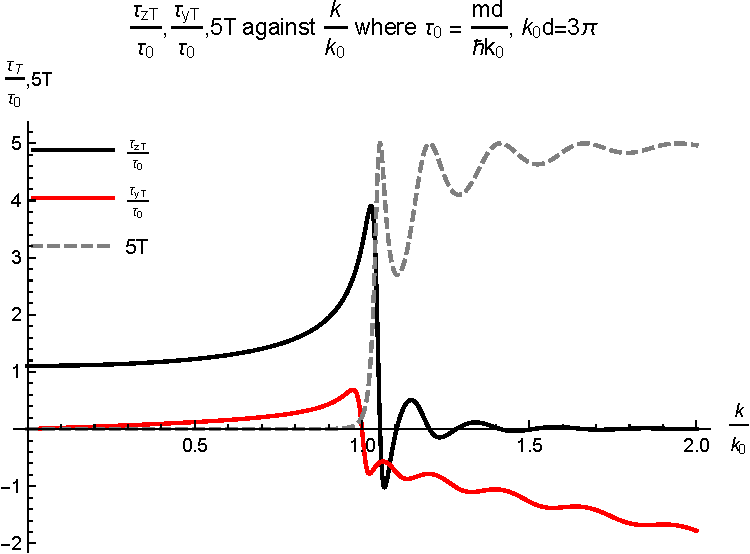
\includegraphics{plot3.pdf}
\caption{Dependence of the characteristic transmission times and transmission probability on wavenumber.}
\label{fig:tzvst01}
\end{figure}

\noindent One can define characteristic reflection times $\tau_{zR}, \tau_{yR}, \tau_{xR}$ analogous to those in (\ref{characteristictransmissiontimes}) such that:

\begin{subequations}
\begin{align}
	\langle S_z \rangle_R &= \frac{\hbar}{2}\omega_L\tau_{zR} \\
	\langle S_y \rangle_R &= -\frac{\hbar}{2}\omega_L\tau_{yR} \\
	\langle S_x \rangle_R &= \frac{\hbar}{2}\left(1-\frac{\omega_L^2\tau_{xR}^2}{2}\right)
\end{align}
\end{subequations}

\noindent By application of equations (\ref{stsrrelations}), one arrives at:

\begin{subequations}
\begin{align}
	\tau_{zR}&=-\tau_{zT} \frac{T}{R}\\
	\tau_{yR}&=\tau_{yT}\\
\tau_{xR}&=(\tau_{yR}^2+\tau_{zR}^2)^{\frac{1}{2}}=\left(\tau_{yT}^2+\tau_{zT}^2 \frac{T^2}{R^2}\right)^{\frac{1}{2}}
\end{align}
\end{subequations}

\pagebreak
\section{Tunnelling Times in the de Broglie-Bohm Interpretation}
\label{section:dBB}
\subsection{de Broglie-Bohm Theory}
\label{subsection:dBBtheory}
\noindent It is clear from the previous section that no definitive answer to the equation \textit{`How long does a particle take to tunnel through a quantum barrier'} has been agreed upon within the orthodox interpretation of quantum mechanics. In contrast, the de Broglie-Bohm (dBB) interpretation yields a unique and well-defined prescription for defining tunnelling times. The dBB theory is an interpretation of quantum mechanics built upon the following postulates (Holland (1993)):

\begin{itemize}
\item [P1] Individual physical systems comprise a wave propagating in space and time, and a point particle, the motion of which is guided by the wave.
\item [P2] The wave is mathematically described by $\psi(t,\boldsymbol{y}) = Re^{iS/\hbar}, R=R(t,\boldsymbol{y}) \text{ is a real amplitude function, } \\S=S(t,\boldsymbol{y}) \text{ is a real phase function and} \psi(t,\boldsymbol{y}) \text{ satisfies the time dependent Schr{\"o}dinger equation.}$
\item [P3] The velocity of the particle is given by $\boldsymbol{v} = \frac{1}{m}\nabla{S}$. The particle motion is obtained by solving this equation along with the specification of the initial condition of the particle, $\boldsymbol{y}(0)$.
\item [P4] The probability of a particle \textit{being} between points $\boldsymbol{y} \text{ and } \boldsymbol{y + dy}$ at time $t$ is given by:
\begin{equation}
	|\psi(t,\boldsymbol{y})|^2d^3y = R(t,\boldsymbol{y})^2d^3y
\end{equation}
The effect of this postulate is to extract from all possible motions of the particle those compatible with the initial distribution $R(0,\boldsymbol{y})$. Note how this differs from the orthodox interpretation in which $|\psi(t,\boldsymbol{y})|^2$ determines the probability density of finding a particle \textit{upon measurement}.
\end{itemize}

\noindent Substituting in $\psi = Re^{iS/\hbar}$ into the time dependent Schr{\"o}dinger equation yields:

\begin{subequations}
\begin{align}
	&\frac{\partial S}{\partial t}+\frac{(\nabla S)^2}{2m}-\frac{\hbar^2}{2m}\frac{\nabla^2 R}{R}+V=0 \label{dBBHJ} \\
	&\frac{\partial R^2}{\partial t}+\nabla\cdot\left(\frac{R^2\nabla S}{m}\right)=0 \label{dBBcontinuity}
\end{align}
\end{subequations}

\begin{proof}
\begin{subequations}
\begin{align}
i\hbar \frac{\partial\psi}{\partial t} &= \frac{-\hbar^2}{2m}\nabla^2\psi+V\psi\\
i\hbar\left(\dot{R}+\frac{i}{\hbar}R\dot{S}\right) &= -\frac{\hbar^2}{2m}\left(\nabla^2R+\frac{2i}{\hbar}\nabla R \nabla S-\frac{1}{\hbar^2}R(\nabla S)^2+\frac{i}{\hbar}R\nabla^2 S\right)+VR\\\intertext{Isolating real and imaginary parts yields:}
-R\dot{S}&=-\frac{\hbar^2}{2m}\left(\nabla^2 R-\frac{R}{\hbar^2}(\nabla S)^2\right)+VR&\\
\implies &\frac{\partial S}{\partial t}+\frac{(\nabla S)^2}{2m}-\frac{\hbar^2}{2m}\frac{\nabla^2 R}{R}+V=0\\
\hbar\dot{R} &= -\frac{\hbar}{2m}\left(2\nabla R\nabla S+R\nabla^2S\right)\\
\implies &\frac{\partial R^2}{\partial t}+\nabla\cdot\left(\frac{R^2\nabla S}{m}\right)=0
\end{align}
\end{subequations}
\end{proof}

\noindent Note that (\ref{dBBcontinuity}) can be written as:

\begin{equation}
	\frac{\partial P(t,\boldsymbol{y})}{\partial t}+\nabla \cdot \boldsymbol{j}(t,\boldsymbol{y})=0
\end{equation}

\noindent where $P$ is the probability density and $\boldsymbol{j}$ is the 3-dimensional generalisation of the flux (\ref{1dflux}), and hence takes the form of the continuity equation. Note also equation (\ref{dBBHJ}) is a modified Hamilton-Jacobi equation, with additional term $Q=-\frac{\hbar^2}{2m}\frac{\nabla^2 R}{R}$, the `quantum potential energy'.

\noindent As in P3 one defines the vector field $\boldsymbol{v} = \frac{1}{m}\nabla S$, which defines at each point in space at each instant in time the tangent to the particle's trajectory passing through that point. Given the gradient $\nabla S$ is orthogonal to level surfaces, the trajectories are orthogonal to surfaces $S=constant$, and are given by the solution of $\dot{\boldsymbol{y}}=\frac{1}{m}\nabla S(t,\boldsymbol{y})$, requiring specification of the initial condition $\boldsymbol{y}_0$. Hence the motion of the particle is completely deterministic once its initial position has been specified. Note one does not have to specify an initial velocity $\boldsymbol{v}_0$ as this is encoded in the initial wave $\psi_0(\boldsymbol{y})$ and is calculated using P2. Note also the important fact that no two different trajectories with the same wave $\psi(t,\boldsymbol{y})$ intersect. This is because at the point of intersection, both trajectories have the same velocity and position at the same point in time. As the motion of a particle is deterministic given the specification of an initial condition, the two trajectories will subsequently coincide for all times after the time of intersection. By time reversal invariance, the two trajectories must also have coincided for all anticedent times, a contradiction with our initial assumption.

From P3 it is clear that an ensemble of possible motions associated with the same wave is generated by varying the initial condition $\boldsymbol{y}_0$. Once specified, the laws governing the evolution of a physical system are entirely deterministic. The probabilistic nature of quantum mechanics, familiar from experiments such as the double-slit experiment, is recovered from the fact that giving a particle a precisely defined initial condition is empirically unrealisable. Hence given an ensemble of identical physical systems (a wave and point particle), it is the uncertainty of the initial position of the particles that gives rise to the probabilistic nature of quantum mechanics. 

\subsection{A Natural Definition of Tunnelling Time}
\label{subsection:dBBtime}

The notion of a particle trajectory in the dBB theory leads one to a natural definition of reflection and transmission times. For a particle with initial condition (restricting to the one-dimensional case) $y=y_0$ at $t=0$, the time spent in the region $y_1 \leq y \leq y_2$ is given by:

\begin{equation}
	t(y_0;y_1,y_2) = \int_0^\infty dt \Theta(y(t,y_0)-y_1)\Theta(y_2-y(t,y_0)) \label{tclassical}
\end{equation}

\noindent where $y(t,y_0)$ denotes the trajectory of a particle with initial condition $y=y_0 \text{ at } t=0$ and $\Theta$ is the Heaviside step function. This definition is intuitively clear: $\Theta(y(t,y_0)-y_1)$ has support for particle trajectories $> y_1$, and $\Theta(y_2-y(t,y_0)$ has support for particle trajectories $<y_2$. When a trajectory satisfies both of these conditions, the particle resides within the interval of interest $(y_1,y_2)$ and increments the measured time.

For empirical purposes, the precise specification of the particle's initial condition is not possible. For an ensemble of identical systems, one can use P4 at $t=0$ to state the probability distribution of initial positions, and hence define the mean dwell time:

\begin{subequations}
\begin{flalign}
	\tau_D(y_1,y_2) &= \langle t(y_0;y_1,y_2) \rangle = \int_{-\infty}^{\infty}dy_{0}|\psi(0,y_0)|^2t(y_0;y_1,y_2)&\\
			&\stackrel{\mathclap{(\ref{tclassical})}}{=} \int_{-\infty}^{\infty}dy_{0}|\psi(0,y_0)|^2 \int_0^\infty dt \Theta(y(t,y_0)-y_1)\Theta(y_2-y(t,y_0)) \\
			&= \int_{-\infty}^{\infty}dy_{0}|\psi(0,y_0)|^2 \int_0^\infty dt \int_{-\infty}^\infty \Theta(y-y_1)\Theta(y_2-y)\delta(y-y(t,y_0))\\
			&= \int_0^\infty \int_{y_1}^{y_2} \int_{-\infty}^\infty dy_{0}|\psi(0,y_0)|^2\delta(y-y(t,y_0))\\
			&= \int_0^\infty \int_{y_1}^{y_2}|\psi(t,y)|^2
\end{flalign}
\end{subequations}

\noindent where $|\psi(t,y)|^2 = \langle \delta(y-y(t,y_0)) \rangle$. Leavens and Aers (1989 pp. 1204) argue this to be identical to the time derived above (\ref{dwelltimedef}).

One can use the fact that particle trajectories do not intersect each other to define a starting point $y_0^c$ such that only trajectories $y(t,y_0)$ with $y_0 > y_0^c$ are ultimately transmitted, and trajectories with $y_0 < y_0^c$ are ultimately reflected. $y_0^c$ is defined by:

\begin{equation}
	\int_{y_0^c}^\infty dy_0 |\psi(0,y_0)|^2=|T|^2
\end{equation}

\noindent This definition is intuitively clear - the left hand side is the probability a particle starts in a region that guarantees it will be ultimately transmitted, and this is equal to the transmission probability.

\begin{figure}[ht]
    \centering
    \incfig{Trajectory}
    \caption{$y_0^c$ separates reflected and transmitted trajectories.}
    \label{fig:trajectories}
\end{figure}

\noindent Subsequently one can calculate the mean transmission and reflection times, uniquely given by:

\begin{align}
	\tau_T(y_1,y_2)&=\frac{\langle(t(y_0;y_1,y_2)\Theta(y_0-y_0^c)\rangle}{\langle\Theta(y_0-y_0^c)\rangle}\\
	\tau_R(y_1,y_2)&=\frac{\langle(t(y_0;y_1,y_2)\Theta(y_0^c-y_0)\rangle}{\langle\Theta(y_0^c-y_0)\rangle}.
\end{align}

\noindent where $|T|^2 = \langle\Theta(y_0-y_0^c)\rangle \text{ and } |R|^2 = \langle\Theta(y_0^c-y_0)\rangle$. These are real-valued, non-negative quantities obeying the consistency condition (\ref{dwellcondition}):

\begin{subequations}
\begin{align}
	|T|^2\tau_T(y_1,y_2)+|R|^2\tau_R(y_1,y_2) &= \langle(t(y_0;y_1,y_2)\Theta(y_0-y_0^c)\rangle+\langle(t(y_0;y_1,y_2)\Theta(y_0^c-y_0)\rangle\\
						  &= \langle(t(y_0;y_1,y_2)(\Theta(y_0-y_0^c)+\Theta(y_0^c-y_0))\rangle\\
						  &= \langle t(y_0;y_1,y_2) \rangle = \tau_D
\end{align}
\end{subequations}

\noindent The probability distributions of the transmission and reflection times,$P_T \text{ and } P_R$ are also of interest. These are defined by:

\begin{equation}
	\tau_T(y_1,y_2) = \int_0^\infty dt P_T(t(y_1,y_2))t, \quad \tau_R(y_1,y_2) = \int_0^\infty dt P_R(t(y_1,y_2))t.
\end{equation}

\noindent and hence are given by

\begin{subequations}
\begin{align}
	P_T(t(y_1,y_2))&:=\frac{\langle(\Theta(y_0-y_0^c))\delta[t(y_1,y_2)-t(y_0;y_1,y_2)]\rangle}{\langle\Theta(y_0-y_0^c)\rangle}\\
	P_R(t(y_1,y_2))&:=\frac{\langle(\Theta(y_0^c-y_0))\delta[t(y_1,y_2)-t(y_0;y_1,y_2)]\rangle}{\langle\Theta(y_0^c-y_0)\rangle}
\end{align}
\end{subequations}

\subsection{Numerical Example}
\label{subsection:dBBexample}
\noindent Consider tunnelling through barrier with boundaries shifted to $[0, d]$ and an electron with initial Gaussian wave function:

\begin{equation}
	\psi(t=0,y) = \frac{1}{(2\pi(\Delta y)^2)^{\frac{1}{4}}}exp\left(-\left(\frac{(y-y_0)^2}{2\Delta y}\right)^2+ik_0y\right)
\end{equation}

\noindent where $y_0$ is the centroid of $|\psi(0,y)|^2$ and $k_0$ is the centroid of $|\phi(k)|^2$, the Fourier transform of the wave function into momentum space. This is a minimum-uncertainty product wave function and hence the uncertainties of its position and momentum satisfy $\Delta y\Delta p_y = \frac{1}{2} (\hbar = 1)$. Note that $y_0$ is chosen such that the wave function is sufficiently far to the left of the barrier region $0\leq y\leq d$ such that the initial probability density $|\psi(0,y)|^2$ is negligible for $y \geq 0$. Mathematically this is formulated as:

\begin{equation}
	\int_0^\infty dy |\psi(0,y)|^2 = 10^{-4}|T|^2
\end{equation}

\noindent The barrier has height $V_0 = 10eV$ and unfixed width d. The problem is solved numerically. For $E_0 = \frac{1}{2}V_0$, momenta uncertainties $\Delta k = 0.04 \text{ and } 0.08 \text{{\AA}}$ and trajectory starting points $y_0$ near the transmission-reflection bifurcation point $y_0^c$, a collection of results are presented below:

\begin{figure}[ht]
    \centering
    \incfigsize{LAcombined2}{15}
    \caption{$y_0^c$ separates reflected and transmitted trajectories.}
    \label{fig:trajectories111wrwd}
\end{figure}



\clearpage

\begin{thebibliography}{100}
\bibitem{Goldstein}
Goldstein, H., Safko, J.L., Poole, C.P. (2002), \textit{Classical Mechanics} (3rd ed.), Addison-Wesley

\bibitem{Hilgevoord}
Hilgevoord, J. (2002), Time in quantum mechanics, \textit{American Journal of Physics} \textbf{70}, 301-306

\bibitem{Sakurai}
Sakurai, J.J., Napolitano, J.J. (2017), \textit{Modern Quantum Mechanics}, Cambridge University Press

\bibitem{Buttiker}
B{\"u}ttiker, M. (1983), Larmor precession and the traversal time for tunnelling, \textit{Physical Review B} \textbf{27}, 6178-6188

\bibitem{LeavensA}
Leavens, C.R. (1996), The “tunneling-time problem” for electrons, in \textit{Bohmian Mechanics and Quantum Theory: An Appraisal}, Cushing J.T., Fine A., Goldstein S. (eds), Springer

\bibitem{LeavensB}
Leavens, C.R. (1990), Traversal times for rectangular barriers within Bohm's causal interpretation of quantum mechanics, \textit{Solid State Communications} \textbf{76}, 253-261

\bibitem{HandS}
Hauge, E. and St{\o}vneng J. (1989), Tunneling times: a critical review, \textit{Reviews of Modern Physics} \textbf{61}, 917–936

\bibitem{LandA}
Leavens, C.R., Aers, G.C. (1989), Dwell time and phase times for transmission and reflection, \textit{Physical Review B} \textbf{39}, 1202-1206

\bibitem{LandA2}
Leavens, C.R., Aers, G.C. (1990), Tunnelling times for one-dimensional barriers, in \textit{Scanning Tunnelling Microscopy and Related Mathods}, Behm R.J., Garcia N., Rohrer H. (eds), Springer

\bibitem{Peres}
Peres, A. (1980), Measurement of time by quantum clocks, \textit{American Journal of Physics} \textbf{48}, 552–557

\bibitem{Holland}
Holland, P.R. (1993), \textit{The Quantum Theory of Motion}, Cambridge University Press



\end{thebibliography}
\end{document}
